\documentclass[11pt,]{article}
\usepackage{lmodern}
\usepackage{amssymb,amsmath}
\usepackage{ifxetex,ifluatex}
\usepackage{fixltx2e} % provides \textsubscript
\ifnum 0\ifxetex 1\fi\ifluatex 1\fi=0 % if pdftex
  \usepackage[T1]{fontenc}
  \usepackage[utf8]{inputenc}
\else % if luatex or xelatex
  \ifxetex
    \usepackage{mathspec}
    \usepackage{xltxtra,xunicode}
  \else
    \usepackage{fontspec}
  \fi
  \defaultfontfeatures{Mapping=tex-text,Scale=MatchLowercase}
  \newcommand{\euro}{€}
\fi
% use upquote if available, for straight quotes in verbatim environments
\IfFileExists{upquote.sty}{\usepackage{upquote}}{}
% use microtype if available
\IfFileExists{microtype.sty}{%
\usepackage{microtype}
\UseMicrotypeSet[protrusion]{basicmath} % disable protrusion for tt fonts
}{}
\usepackage[margin=1.0in]{geometry}
\ifxetex
  \usepackage[setpagesize=false, % page size defined by xetex
              unicode=false, % unicode breaks when used with xetex
              xetex]{hyperref}
\else
  \usepackage[unicode=true]{hyperref}
\fi
\hypersetup{breaklinks=true,
            bookmarks=true,
            pdfauthor={},
            pdftitle={De novo clustering methods out-perform reference-based methods for assigning 16S rRNA gene sequences to operational taxonomic units},
            colorlinks=true,
            citecolor=blue,
            urlcolor=blue,
            linkcolor=magenta,
            pdfborder={0 0 0}}
\urlstyle{same}  % don't use monospace font for urls
\setlength{\parindent}{0pt}
\setlength{\parskip}{6pt plus 2pt minus 1pt}
\setlength{\emergencystretch}{3em}  % prevent overfull lines
\providecommand{\tightlist}{%
  \setlength{\itemsep}{0pt}\setlength{\parskip}{0pt}}
\setcounter{secnumdepth}{0}

%%% Use protect on footnotes to avoid problems with footnotes in titles
\let\rmarkdownfootnote\footnote%
\def\footnote{\protect\rmarkdownfootnote}

%%% Change title format to be more compact
\usepackage{titling}

% Create subtitle command for use in maketitle
\newcommand{\subtitle}[1]{
  \posttitle{
    \begin{center}\large#1\end{center}
    }
}

\setlength{\droptitle}{-2em}
  \title{\textbf{\emph{De novo} clustering methods out-perform reference-based
methods for assigning 16S rRNA gene sequences to operational taxonomic
units}}
  \pretitle{\vspace{\droptitle}\centering\huge}
  \posttitle{\par}
  \author{}
  \preauthor{}\postauthor{}
  \date{}
  \predate{}\postdate{}

\usepackage{helvet} % Helvetica font
\renewcommand*\familydefault{\sfdefault} % Use the sans serif version of the font
\usepackage[T1]{fontenc}

\usepackage[none]{hyphenat}
\usepackage[all]{nowidow}

\usepackage{setspace}
\doublespacing
\setlength{\parskip}{1em}

\usepackage{lineno}

\usepackage{pdfpages}

% Redefines (sub)paragraphs to behave more like sections
\ifx\paragraph\undefined\else
\let\oldparagraph\paragraph
\renewcommand{\paragraph}[1]{\oldparagraph{#1}\mbox{}}
\fi
\ifx\subparagraph\undefined\else
\let\oldsubparagraph\subparagraph
\renewcommand{\subparagraph}[1]{\oldsubparagraph{#1}\mbox{}}
\fi

\begin{document}
\maketitle

\begin{center}
\vspace{25mm}
Sarah L. Westcott and Patrick D. Schloss${^\dagger}$

\vspace{30mm}

$\dagger$ To whom correspondence should be addressed: pschloss@umich.edu

Department of Microbiology and Immunology, University of Michigan, Ann Arbor, MI
\end{center}

\newpage

\linenumbers

\subsection{Abstract}\label{abstract}

\textbf{Background.} 16S rRNA gene sequences are routinely assigned to
operational taxonomic units (OTUs) that are then used to analyze complex
microbial communities. A number of methods have been employed to carry
out the assignment of 16S rRNA gene sequences to OTUs leading to
confusion over which method is optimal. A recent study suggested that a
clustering method should be selected based on its ability to generate
stable OTU assignments that do not change as additional sequences are
added to the dataset. In contrast, we contend that the quality of the
OTU assignments, the ability of the method to properly represent the
distances between the sequences, is more important.

\textbf{Methods.} Our analysis implemented six \emph{de novo} clustering
algorithms including the single linkage, complete linkage, average
linkage, abundance-based greedy clustering, distance-based greedy
clustering, and Swarm and the open and closed-reference methods. Using
two previously published datasets we used the Matthew's Correlation
Coefficient (MCC) to assess the stability and quality of OTU
assignments.

\textbf{Results.} The stability of OTU assignments did not reflect the
quality of the assignments. Depending on the dataset being analyzed, the
average linkage and the distance and abundance-based greedy clustering
methods generated OTUs that were more likely to represent the actual
distances between sequences than the open and closed-reference methods.
We also demonstrated that for the greedy algorithms VSEARCH produced
assignments that were comparable to those produced by USEARCH making
VSEARCH a viable free and open source alternative to USEARCH. Further
interrogation of the reference-based methods indicated that when USEARCH
or VSEARCH were used to identify the closest reference, the OTU
assignments were sensitive to the order of the reference sequences
because the reference sequences can be identical over the region being
considered. More troubling was the observation that while both USEARCH
and VSEARCH have a high level of sensitivity to detect reference
sequences, the specificity of those matches was poor relative to the
true best match.

\textbf{Discussion.} Our analysis calls into question the quality and
stability of OTU assignments generated by the open and closed-reference
methods as implemented in current version of QIIME. This study
demonstrates that \emph{de novo} methods are the optimal method of
assigning sequences into OTUs and that the quality of these assignments
needs to be assessed for multiple methods to identify the optimal
clustering method for a particular dataset.

\newpage

\subsection{Introduction}\label{introduction}

The ability to affordably generate millions of 16S rRNA gene sequences
has allowed microbial ecologists to thoroughly characterize the
microbial community composition of hundreds of samples. To simplify the
complexity of these large datasets, it is helpful to cluster sequences
into meaningful bins. These bins, commonly known as operational
taxonomic units (OTUs), are used to compare the biodiversity contained
within and between different samples (Schloss \& Westcott, 2011). Such
comparisons have enabled researchers to characterize the microbiota
associated with the human body (e.g. Huttenhower et al., 2012), soil
(e.g. Shade et al., 2013), aquatic ecosystems (e.g. Gilbert et al.,
2011), and numerous other environments. Within the field of microbial
ecology, a convention has emerged where sequences are clustered into
OTUs using a threshold of 97\% similarity or a distance of 3\%. One
advantage of the OTU-based approach is that the definition of the bins
is operational and can be changed to suit the needs of the particular
project. However, with the dissemination of clustering methods within
software such as mothur (Schloss et al., 2009), QIIME (Caporaso et al.,
2010), and other tools (Sun et al., 2009; Edgar, 2010, 2013; Cai \& Sun,
2011; Mahé et al., 2014), it is important to understand how different
clustering methods implement this conventional OTU threshold.
Furthermore, it is necessary to understand how the selected method
affects the precision and accuracy of assigning sequences to OTUs.
Broadly speaking, three approaches have been developed to assign
sequences to OTUs:

The first approach has been referred to as phylotyping (Schloss \&
Westcott, 2011) or closed reference clustering (Navas-Molina et al.,
2013). This approach involves comparing sequences to a curated database
and then clustering sequences into the same OTU that are similar to the
same reference sequence. Reference-based clustering methods suffer when
the reference does not adequately reflect the biodiversity of the
community. If a large fraction of sequences are novel, then they cannot
be assigned to an OTU. In addition, the reference sequences are selected
because they are less than 97\% similar to each other over the full
length of the gene; however, it is known that the commonly used variable
regions within the 16S rRNA gene do not evolve at the same rate as the
full-length gene (Schloss, 2010; Kim, Morrison \& Yu, 2011). Thus, a
sequence representing a fragment of the gene may be more than 97\%
similar to multiple reference sequences. Defining OTUs in the
closed-reference approach is problematic because two sequences might be
97\% similar to the same reference sequence, but they may only be 94\%
similar to each other. Alternatively, a sequence may be equally similar
to two or more reference sequences. A alternative to this approach is to
use a classifier to assign a taxonomy to each sequence so that sequences
can be clustered at a desired level within the Linnean taxonomic
hierarchy (Schloss \& Westcott, 2011). The strengths of the
reference-based methods include their speed, potential for trivial
parallelization, ability to compare OTU assignments across studies, and
the hope that as databases improve, the OTU assignments will also
improve.

The second approach has been referred to as distance-based (Schloss \&
Westcott, 2011) or \emph{de novo} clustering (Navas-Molina et al.,
2013). In this approach, the distance between sequences is used to
cluster sequences into OTUs rather than the distance to a reference
database. In contrast to the efficiency of closed-reference clustering,
the computational cost of hierarchical \emph{de novo} clustering methods
scales quadratically with the number of unique sequences. The expansion
in sequencing throughput combined with sequencing errors inflates the
number of unique sequences resulting in the need for large amounts of
memory and time to cluster the sequences. If error rates can be reduced
through stringent quality control measures, then these problems can be
overcome (Kozich et al., 2013). As an alternative, heuristics have been
developed to approximate the clustering of hierarchical methods (Sun et
al., 2009; Edgar, 2010; Mahé et al., 2014). Two related heuristics
implemented in USEARCH were recently described: distance-based greedy
clustering (DGC) and abundance-based greedy clustering (AGC) (Edgar,
2010; He et al., 2015). These greedy methods cluster sequences within a
defined similarity threshold of an index sequence or creates a new index
sequence. If a sequence is more similar than the defined threshold, it
is assigned to the closest centroid based (i.e.~DGC) or the most
abundant centroid (i.e.~AGC). One critique of \emph{de novo} approaches
is that OTU assignments are sensitive to the input order of the
sequences (Mahé et al., 2014; He et al., 2015). Whether the differences
in assignments is meaningful is unclear and the variation in results
could represent equally valid clustering of the data. The strength of
\emph{de novo} clustering is its independence of references for carrying
out the clustering step. For this reason, \emph{de novo} clustering has
been preferred across the field. After clustering, the classification of
each sequence can be used to obtain a consensus classification for the
OTU (Schloss \& Westcott, 2011).

The third approach, open-reference clustering, is a hybrid of the
closed-reference and \emph{de novo} approaches (Navas-Molina et al.,
2013; Rideout et al., 2014). Open-reference clustering involves
performing closed-reference clustering followed by \emph{de novo}
clustering on those sequences that are not sufficiently similar to the
reference. In theory, this method should exploit the strengths of both
closed-reference and \emph{de novo} clustering; however, the different
OTU definitions employed by commonly used closed-reference and \emph{de
novo} clustering implementations pose a possible problem when the
methods are combined. An alternative to this approach has been to
classify sequences to a bacterial family or genus and then assign those
sequences to OTUs within those taxonomic groups using the average
linkage method (Schloss \& Westcott, 2011). For example, all sequences
classified as belonging to the \emph{Porphyromonadaceae} would then be
assigned to OTUs using the average linkage method using a 3\% distance
threshold. Those sequences that did not classify to a known family would
also be clustered using the average linkage method. An advantage of this
approach is that it lends itself nicely to parallelization since each
taxonomic group is seen as being independent and can be processed
separately. Such an approach would overcome the difficulty of mixing OTU
definitions between the closed-reference and \emph{de novo} approaches;
however, it would still suffer from the problems associated with
database quality and classification error.

The growth in options for assigning sequences using each of these three
broad approaches has been considerable. It has been difficult to
objectively assess the quality of OTU assignments. Some have focused on
the time and memory required to process a dataset (Sun et al., 2009; Cai
\& Sun, 2011; Mahé et al., 2014; Rideout et al., 2014). These are valid
parameters to assess when judging a clustering method, but have little
to say about the quality of the OTU assignments. Others have attempted
to judge the quality of a method by its ability to generate data that
parallels classification data (White et al., 2010; Sun et al., 2011; Cai
\& Sun, 2011). This approach is problematic because bacterial taxonomy
often reflects historical biases amongst bacterial systematicists.
Furthermore, it is well known that the rates of evolution across
lineages are not the same (Wang et al., 2007; Schloss, 2010). A related
approach has used clustering of mock community data to evaluate methods
(Huse et al., 2010; Barriuso, Valverde \& Mellado, 2011; Bonder et al.,
2012; Chen et al., 2013; Edgar, 2013; Mahé et al., 2014; May et al.,
2014). Yet these approaches ignore the effects of sequencing errors that
tend to accumulate with sequencing depth and represent highly idealized
communities that lack the phylogenetic diversity of real microbial
communities (Schloss, Gevers \& Westcott, 2011; Kozich et al., 2013).
Others have assessed the quality of clustering based on their ability to
generate the same OTUs generated by other methods (Rideout et al., 2014;
Schmidt, Rodrigues \& Mering, 2014b). This is problematic because it
does not solve the fundamental question of which method is optimal. The
concept of ecological consistency as a metric of quality asserts that
sequences that cluster into the same OTU should share similar ecological
affiliations (Koeppel \& Wu, 2013; Preheim et al., 2013; Schmidt,
Rodrigues \& Mering, 2014a). Although this is an intriguing approach and
is a quantitative metric, it is unclear how the metric would be
objectively validated. We recently proposed an approach for evaluating
OTU assignments using the distances between pairs of sequences (Schloss
\& Westcott, 2011). We were able to synthesize the relationship between
OTU assignments and the distances between sequences using the Matthew's
correlation coefficient (MCC; Matthews, 1975). MCC is can be interpreted
as representing the correlation between the observed and expected
classifications and can vary between -1.0 and 1.0. The strength of the
MCC, as implemented by Schloss et al. (2011), is that it is an objective
approach to assessing the quality of the OTU assignments that can be
calculated for any set of OTU assignments where there is a distance
matrix and a specific threshold without relying on an external
reference.

A recent analysis by He and colleagues (2015) characterized the three
general clustering approaches by focusing on what they called stability.
They defined stability as the ability of a method to provide the same
clustering on a subset of the data as was found in the full dataset.
Their concept of stability did not account for the quality of the OTU
assignments and instead focused on the precision of the assignments. A
method may be very stable, but of poor quality. In the current analysis,
we assessed the quality and stability of the various clustering methods.
Building on our previous analysis of clustering methods, our hypothesis
was that the methods praised by the He study for their stability
actually suffered a lack of quality. In addition, we assess these
parameters in light of sequence quality using the original 454 dataset
and a larger and more modern dataset generated using the MiSeq platform.

\subsection{Results and Discussion}\label{results-and-discussion}

\textbf{\emph{Summary and replication of He study.}} We obtained the
Canadian soil dataset from Roesch et al. (2007) and processed the
sequences as described by He and colleagues. Using these data, we
reconsidered three of the more critical analyses performed in the He
study.

First, we sought to quantify whether the OTU assignments observed for a
subset of the data represented the same assignments that were found with
the full dataset. The He study used the MCC to quantify the degree to
which pairs of sequences were in the same OTUs in subsampled and full
datasets. A more robust approach would utilize metrics that quantify the
mutual information held between two sets of clusterings and has been
applied to assess inter-method variation in OTU composition (Schmidt,
Rodrigues \& Mering, 2014b). To maintain consistency with the original
He study, we also calculated the MCC value as they described. The He
study found that when they used the open and closed-reference methods
the OTUs formed using the subsetted data most closely resembled those of
the full dataset. Among the \emph{de novo} methods they observed that
the AGC method generated the most stable OTUs followed by the single
linkage (SL), DGC, complete linkage (CL), and average linkage (AL)
methods. We first calculated the MCC for the OTU assignments generated
by each of the clustering methods using 20, 40, 60, and 80\% of the
sequences relative to the OTU composition formed by the methods using
the full dataset (see Methods for description; Figure 1A). Similar to
the He study, we replicated each method and subsampled to the desired
fraction of the dataset 30 times. Multiple subsamplings were necessary
because a random number generator is used in some of the methods to
break ties where pairs of sequences have the same distance between them.
Across these sequencing depths, we observed that the stability of the
OTUs generated by the SL and CL methods were highly sensitive to
sampling effort relative to the OTUs generated by the AL, AGC, and DGC
methods (Figure 1A). Our results (Figure 1B) largely confirmed those of
Figure 4C in the He study with one notable exception. The He study
observed a broad range of MCC values among their AL replicates when
analyzing OTUs generated using 60\% of the data. This result appeared
out of character and was not explained by the authors. They observed a
mean MCC value of approximately 0.63 (95\% confidence interval between
approximately 0.15 and 0.75). In contrast, we observed a mean value of
0.93 (95\% confidence interval between 0.91 and 0.95). This result
indicates that the AL assignments were far more stable than indicated in
the He study. Regardless, although the assignments are quite stable, it
does support the assertion that the OTU assignments observed for the
subset of the data do not perfectly match the assignments that were
found with the full dataset as they did with the reference-based
methods; however, the significance of these differences is unclear.

Second, the He study and the original Roesch study showed that
rarefaction curves calculated using CL-generated OTU assignments
obtained using a subsample of the sequencing data did not overlap with
rarefaction curves generated using OTU assignments generated from the
full dataset. The He and Roesch studies both found that the CL method
produced fewer OTUs in the subset than in the rarefied data. In
addition, the He study found that the SL method produced more OTUs, the
AGC produced fewer, and the other methods produced similar numbers of
OTUs than expected when comparing the subsetted data to the rarefied
data. Our results support those of these previous studies (Figure 2). It
was clear that inter-method differences were generally more pronounced
than the differences observed between rarefying from the full dataset
and from clustering the subsetted data. The number of OTUs observed was
largest using the CL method, followed by the open-reference method. The
AL, AGC, and DGC methods all provided comparable numbers of OTUs.
Finally, the closed-reference and SL methods generated the fewest number
of OTUs.

Third, the authors attempted to describe the effects of the OTU
assignment instability on comparisons of communities. They used Adonis
to test whether the community structure represented in subsetted
communities resembled that of the full dataset when only using the
unstable OTUs (Anderson, 2001). Although they were able to detect
significant p-values, they appeared to be of marginal biological
significance. Adonis R statistics close to zero indicate the community
structures from the full and subsetted datasets overlapped while values
of one indicate the communities are completely different. The He study
observed adonis R statistics of 0.02 (closed-reference), 0.03
(open-reference), 0.07 (CL, AGC, DGC), and 0.16 (SL and AL). Regardless
of the statistical or biological significance of these results, the
analysis was tautological since, by definition, representing communities
based on their unstable OTUs would yield differences. Furthermore, the
\emph{de novo} and open-reference approaches do not consistently label
the OTUs that sequences belong to when the clustering methods are run
multiple times with different random number seeds. To overcome this, the
authors selected representative sequences from each OTU and used those
representative sequences to link OTU assignments between the different
sized sequence sets. It was not surprising that the only analysis that
did not provide a significant p-value was for the closed-reference
analysis, which is the only analysis that provides consistent OTU
labels. Finally, the authors built off of this analysis to count the
number of OTUs that were differentially represented between the
subsetted and full datasets by each method. This entire analysis assumed
that the OTUs generated using the full dataset were correct, which was
an unsubstantiated assumption since the authors did not assess the
quality of the OTU assignments.

This re-analysis of the He study raised five complementary questions.
First, how do the various methods vary in the quality of their OTU
assignments? Second, how generalizable are these results to modern
datasets generated using a large number of sequences that were deeply
sequenced? Third, how does the stability and quality of OTU assignments
generated by new methods compare to those analyzed in the He study?
Fourth, are there open-source alternatives to USEARCH that perform just
as well? Finally, although the stability of reference-based methods did
not appear to be impacted by the input order of the sequences to be
assigned to OTUs, is the stability of reference-based methods impacted
by the order of the reference sequences? In the remainder of the Results
and Discussion section we address each of these questions.

\textbf{\emph{How do the various methods vary in the quality of their
OTU assignments?}} More important than the stability of OTUs is whether
sequences are assigned to the correct OTUs. A method can generate highly
stable OTUs, but the OTU assignments may be meaningless if they poorly
represent the specified cutoff and the actual distance between the
sequences. To assess the quality of OTU assignments by the various
methods, we made use of the pairwise distance between the unique
sequences to count the number of true positives and negatives and the
number of false positives and negatives for each method and sampling
depth. Those pairs of sequences that were similar to each other and
found in the same OTU were called true positives while those that were
similar and found in different OTUs were called false negatives.
Meanwhile, those pairs of sequences that were different from each other
and found in the same OTU were called false positives and those that
were dissimilar and found in different OTUs were called true negatives.
Counting the frequency of these different classes allowed us to judge
how each method balanced the ratio of true positives and negatives to
false positives and negatives using the MCC. We used the average MCC
value as a measure of a method's quality and its variation as a measure
of its consistency. We made three important observations. First, each of
the \emph{de novo} methods varied in how sensitive their MCC values were
to additional sequences (Figure 1C). The SL and CL methods were the most
sensitive; however, the quality of the OTU assignments did not
meaningfully differ when 80 or 100\% of the data were assigned to OTUs
using the \emph{de novo} methods. Second, the AL method had higher MCC
values than the other methods followed by DGC, AGC, CL, open-reference,
and closed-reference, and SL (Figure 1D). Third, with the possible
exception of the CL method, the MCC values for each of the methods only
demonstrated a small amount of variation between runs of the method with
a different ordering of the input sequences. This indicates that
although there may be variation between executions of the same method,
they produced OTU assignments that were of equal quality. Revisiting the
concept of stability, we question the value of obtaining stable OTUs
when the full dataset is not optimally assigned to OTUs. Our analysis
indicates that the most optimal method for assigning the Canadian soils
sequences to OTUs using a 97\% threshold was the AL method.

\textbf{\emph{How generalizable are these results to modern datasets
generated using a large number of sequences that were deeply
sequenced?}} Three factors make the Canadian soil dataset less than
desirable to evaluate clustering methods. First, it was one of the
earliest 16S rRNA gene sequence datasets published using the 454 FLX
platform. Developments in sequencing technology now permit the
sequencing of millions of sequences for a study. In addition, because
the original Phred quality scores and flowgram data are not available,
it was not possible for us to adequately remove sequencing errors
(Schloss, Gevers \& Westcott, 2011). The large number of sequencing
errors that one would expect to remain in the dataset are likely to
negatively affect the performance of all of the clustering methods.
Second, the dataset used in the He study covered the V9 region of the
16S rRNA gene. For a variety of reasons, this region is not well
represented in databases, including the reference database used by the
closed and open-reference methods. Of the 99,322 sequences in the
default QIIME database, only 48,824 fully cover the V9 region. In
contrast, 99,310 of the sequences fully covered the V4 region.
Inadequate coverage of the V9 region would adversely affect the ability
of the reference-based methods to assign sequences to OTUs. Third, our
previous analysis has shown that the V9 region evolves at a rate much
slower than the rest of the gene (Schloss, 2010). With these points in
mind, we compared the clustering assignment for each of these methods
using a time series experiment that was obtained using mouse feces
(Schloss et al., 2012; Kozich et al., 2013). The MiSeq platform was used
to generate 2,825,000 sequences from the V4 region of the 16S rRNA gene
of 360 samples. Parallel sequencing of a mock community indicated that
the sequencing error rate was approximately 0.02\% (Kozich et al.,
2013). Although no dataset is perfect for exhaustively testing these
clustering methods, this dataset was useful for demonstrating several
points. First, when using 60\% of the data, the stability relationships
amongst the different methods were similar to what we observed using the
Canadian soil dataset (Figure 3AB). With the exception for the clusters
generated using CL, the methods all performed very well with stabilities
greater than 0.91. Second, the MCC values calculated relative to the
distances between sequences were generally higher than was observed for
the Canadian soil dataset for all of the methods except the CL and SL
methods. Surprisingly, the MCC values for the DGC (0.77) and AGC (0.76)
methods were comparable to the AL method (0.76; Figure 3CD). This result
suggests that the optimal method is likely to be database-dependent.

Finally, as was observed with the Canadian soil dataset, there was
little variation in MCC values observed among the 30 randomizations.
Therefore, although the methods have a stochastic component, the OTU
assignments did not vary meaningfully between runs. The results from
both the Canadian soil and murine microbiota datasets demonstrate that
the \emph{de novo} methods can generate stable OTU assignments and that
the the overall quality of the assignments were consistent. Most
importantly, these analyses demonstrate that the OTU assignments using
the AL, AGC, and DGC \emph{de novo} methods were consistently better
than either of the reference-based methods.

\textbf{\emph{How does the stability and quality of OTU assignments
generated by new methods compare to those analyzed in the He study?}}
The Swarm algorithm is a recently proposed \emph{de novo} method for
assigning sequences to OTUs that uses user-defined parameters to break
up chains generated by SL clustering (Mahé et al., 2014). Swarm was
originally validated by comparing the results against the expected
clusters formed based on the taxonomic composition of a mock community.
Similar to the authors of the He study, the Swarm developers suggest
that methods are needed that are insensitive to input order. Use of
Swarm on the Canadian soil and murine datasets demonstrated that similar
to the other \emph{de novo} methods, Swarm's OTU assignments changed as
sequences were added (Figures 1A and 3A). When we compared the OTU
assignments for both datasets when using all of the sequence data, the
variation in MCC values across the 30 randomizations were not
meaningfully different (Figures 1D and 3D). Most importantly, when we
selected the distance threshold that optimized the MCC value, the
quality of the OTU assignments was close to that of the AL assignments
when using the Canadian soil dataset and considerably worse than that of
the murine dataset (Figures 1D and 3D). Interestingly, the distance
thresholds that resulted in the largest MCC values were 3 and 2\% for
the Canadian soil and murine datasets, respectively. This suggests that
distance-based OTU definitions are not consistent across datasets when
using the Swarm algorithm, although they do appear to be within the
neighborhood of 3\%. Finally, the Swarm developers indicated that
hierarchical \emph{de novo} algorithms were too impractical to use on
large MiSeq-generated datasets. Our ability to apply AL to the large
mouse dataset and even larger datasets suggests that it is not necessary
to sacrifice OTU assignment quality for speed (e.g. Schubert, Sinani \&
Schloss, 2015; Zackular et al., 2015).

\textbf{\emph{Are there open-source alternatives to USEARCH that perform
just as well?}} For some datasets the AGC and DGC methods appear to
perform as well or better than the hierarchical clustering methods. As
originally described in the He study, the AGC and DGC methods utilized
the USEARCH program and the DGC method is used for clustering in UPARSE
(Edgar, 2010, 2013). The source code for USEARCH is not publicly
available and only the 32-bit executables are available for free to
academic users. Access for non-academic users and those needing the
64-bit version is available commercially from the developer. An
alternative to USEARCH is VSEARCH, which is being developed in parallel
to USEARCH as an open-source alternative. One subtle difference between
the two programs is that USEARCH employs a heuristic to generate
candidate alignments whereas VSEARCH generates the actual global
alignments. The VSEARCH developers claim that this difference enhances
the sensitivity of VSEARCH relative to USEARCH. Using the two datasets,
we determined whether the AGC and DGC methods, as implemented by the two
programs, yielded OTU assignments of similar quality. In general the
overall trends that we observed with the USEARCH-version of AGC and DGC
were also observed with the VSEARCH-version of the methods (Figure 4).
When we compared the two implementations of the AGC and DGC methods, the
OTUs generated by the VSEARCH-version of the methods were as stable or
more stable than the USEARCH-version when using 60\% of the datasets. In
addition, the MCC values for the entire datasets, calculated relative to
the distance matrix, were virtually indistinguishable. These results are
a strong indication that VSEARCH is a suitable and possibly better
option for executing the AGC and DGC methods.

\textbf{\emph{Is the stability of reference-based methods impacted by
the order of the reference sequences?}} The He study and our replication
attempt validated that the closed-reference method generated perfectly
stable OTUs. This was unsurprising since, by definition, the method is
designed to return one-to-one mapping of reads to a reference.
Furthermore, because it treats the input sequences independently the
input order or use of a random number generator is not an issue. An
important test that was not performed in the He study was to determine
whether the clustering was sensitive to the order of the sequences in
the database. The default database used in QIIME, which was also used in
the He study, contains full-length sequences that are at most 97\%
similar to each other. We randomized the order of the reference
sequences 30 times and used them to carry out the closed-reference
method with the full murine dataset, which contained 32,106 unique
sequences (Figure 5). Surprisingly, we observed that the number of OTUs
generated was not the same in each of the randomizations. On average
there were 28,059 sequences that mapped to a reference OTU per
randomization (range from 28,007 to 28,111). The original ordering of
the reference resulted in 27,876 sequences being mapped, less than the
minimum observed number of mapped sequences when the references were
randomized. This surprising result was likely due to the performance of
the USEARCH heuristic. To test this further, we substituted VSEARCH for
USEARCH in the closed-reference method. When we used VSEARCH the
original ordering of the reference sequences and all randomizations were
able to map 27,737 sequences to reference OTUs. When we calculated the
true distance between each of the murine sequences and the references,
we were able to map 28,238 of the murine sequences to the reference
sequences when using a 97\% similarity threshold without the use of a
heuristic. This result indicates that the closed reference approach,
whether using USEARCH or VSEARCH, does not exhaustively or accurately
map reads to the closest reference. To quantify this further, we
calculated the MCC for the USEARCH and VSEARCH assignments relative to
the assignments using the non-heuristic approach. Using USEARCH the
average MCC was 0.78 (range: 0.75 to 0.80) and using VSEARCH the average
MCC was 0.65 (range: 0.64 to 0.66). The two methods had similar
sensitivities (USEARCH: 0.98 and VSEARCH: 0.97), but the USEARCH
specificity (0.73) was considerably higher than VSEARCH (0.60). Overall,
these results indicate that although heuristic approaches may be fast,
they do a poor job of mapping reads to the correct reference sequence
relative to non-heuristic approaches.

We also observed that regardless of whether we used USEARCH or VSEARCH,
the reference OTU labels that were assigned to each OTU differed between
randomizations. When we used USEARCH to perform closed-reference
clustering, an average of 57.38\% of the labels were shared between
pairs of the 30 randomizations (range=56.14 to 59.55\%). If we instead
used VSEARCH an average of 56.23\% of the labels were shared between
pairs of the 30 randomizations (range=53.48 to 59.12\%). To better
understand this result, we further analyzed QIIME's reference database.
We hypothesized that within a given region there would be sequences that
were more than 97\% similar and possibly identical to each other. When a
sequence was used to search the randomized databases, it would encounter
a different reference sequence as the first match with each
randomization. Among the 99,310 reference sequences that fully overlap
the V4 region, there were 7,785 pairs of sequences that were more than
97\% similar to each other over the full length of the 16S rRNA gene.
When the extracted V4 sequences were dereplicated, we identified 88,347
unique sequences. Among these dereplicated V4 sequences there were
311,430 pairs of sequences that were more than 97\% similar to each
other. The presence of duplicate and highly similar V4 reference
sequences explains the lack of labeling stability when using either
USEARCH or VSEARCH to carry out the closed-reference method. We suspect
that the reference database was designed to only include sequences that
were at most 97\% similar to each other as a way to overcome the
limitations of the USEARCH search heuristic.

Beyond comparing the abundance of specific OTUs across samples, the
reference database is used in the open and closed-reference methods to
generate OTU labels that can be used in several downstream applications.
It is commonly used to extract information from a reference phylogenetic
tree to carrying out UniFrac-based analyses (Hamady, Lozupone \& Knight,
2009) and to identify reference genomes for performing analyses such as
PICRUSt (Langille et al., 2013). Because these downstream applications
depend on the correct and unique labeling of the OTUs, the lack of label
stability is problematic. As one illustration of the effects that
incorrect labels would have on an analysis, we asked whether the
duplicate sequences had the same taxonomies. Among the 3,132 V4
reference sequences that had one duplicate, 443 had discordant
taxonomies. Furthermore, among those 1,699 V4 reference sequences with
two or more duplicates, 698 had discordant taxonomies. Two V4 reference
sequences mapped to 30 and 10 duplicate sequences and both contained 7
different taxonomies. Among the V4 sequences within the database, there
was also a sequence that had 131 duplicates and represented 5 different
taxonomies. When we analyzed the 28,238 sequences that mapped to the V4
reference sequences using a non-heuristic approach, we observed that
18,315 of the sequences mapped to more than one reference sequence. Of
these sequences, 13,378 (73.04\%) mapped to references that were
identical over the V4 region and 4,937 (26.96\%) mapped equally well to
two or more references that were not identical over the V4 region. Among
the combined 18,315 sequences that mapped to multiple reference
sequences, the taxonomy of the multiple reference sequences conflicted
for 3,637 (19.86\%). Together, these results demonstrate some of the
considerable problems with the reference-based clustering of sequences.

\subsection{Conclusions}\label{conclusions}

It is worth noting that the analysis from the Roesch study that
motivated the He study is not typical of microbial ecology studies.
First, their analysis was based on a single soil sample. Researchers
generally have dozens or hundreds of samples that are pooled and
clustered together to enable comparison across samples. Second, all of
the sequence data from these datasets is pooled for a single analysis.
Rarely would a researcher rarefy their data prior to clustering since it
can be more efficiently done after all of the data are assigned to OTUs.
Third, the CL method used in the original Roesch study has since been
shown to not generate optimal OTUs (Schloss \& Westcott, 2011). As for
the approach used in the He study, the value of identifying stable OTUs
is unclear. Although there is concern that running the methods multiple
times yields different clusterings, we have shown that there is little
variation in their quality. This suggests that the different clusterings
by the same method are equally good. Greater emphasis should be placed
on obtaining an optimal balance between splitting similar sequences into
separate OTUs and merging disparate sequences into the same OTU.

The approach of the current study quantified the effects of merging and
splitting by using an objective metric. Through the use of the pairwise
distances between sequences, we were able to use the MCC to demonstrate
that, in general, the AL method was consistently the optimal method for
each dataset, but that Swarm, AGC, and DGC sometimes perform as well as
AL. At least for the murine dataset, Swarm also could be among the
methods that performed poorly. It is impossible to obtain a clustering
with no false positives or false negatives and the optimal method may
vary by dataset. With this in mind, researchers are encouraged to
calculate and report their MCC values and to use these values to justify
using methods other than the AL. As an alternative to the He study's
method of measuring stability, we propose using the variation in the
quality of the clustering of the full dataset. Given the tight 95\%
confidence intervals shown in Figures 1D and 3D, with the exception of
CL, it is clear that this variation is quite small. This indicates that
although the order of the sequences being clustered can affect the
actual cluster assignments, the quality of those different clusterings
is not meaningfully different.

Our analysis of those methods that implemented USEARCH as a method for
clustering sequences revealed that its heuristic limited its
specificity. When we replaced USEARCH with VSEARCH, the clustering
quality was as good or better. Although there may be parameters in
USEARCH that can be tuned to improve the heuristic, these parameters are
likely dataset dependent. Based on the data presented in this study, its
availability as an open source, and free program, VSEARCH should replace
USEARCH in the \emph{de novo} clustering methods; however, USEARCH
performed better than VSEARCH for closed-reference clustering.
Furthermore, although not tested in our study, VSEARCH can be
parallelized leading to potentially significant improvements in speed.
Although USEARCH and VSEARCH do not utilize aligned sequences, it is
important to note that a sequence curation pipeline including denoising,
alignment, trimming to a consistent region of the 16S rRNA gene, and
chimera checking are critical to making proper inferences (Schloss,
Gevers \& Westcott, 2011; Schloss, 2012; Kozich et al., 2013).

We have assessed the ability of reference-based clustering methods to
capture the actual distance between the sequences in a dataset in
parallel with \emph{de novo} methods. Several studies have lauded both
the open and closed-reference approaches for generating reproducible
clusterings (Navas-Molina et al., 2013; Rideout et al., 2014; He et al.,
2015), yet we have shown that both reference-based approaches did a poor
job of representing the distance between the sequences compared to the
\emph{de novo} approaches. Although the OTU assignments are reproducible
and stable across a range of library sizes, the reference-based OTU
assignments are a poor representation of the data. We also observed that
the assignments were not actually reproducible when the order of the
reference sequences was randomized. When USEARCH was used, the actual
number of sequences that mapped to the reference changed depended on the
order of the reference. Perhaps most alarming was that the default order
of the database provided the worst MCC of any of the randomizations we
attempted. This has the potential to introduce systematic a bias rather
than a random error. Even when we used VSEARCH to perform
closed-reference clustering and were able to obtain a consistent
clusterings, we observed that the labels on the OTUs differed between
randomizations. Because the OTU labels are frequently used to identify
representative sequences for those OTUs, variation in labels, often
representing different taxonomic groups, will have a detrimental effect
on the interpretation of downstream analyses.

Because the open-reference method is a hybrid of the closed-reference
and DGC methods, it is also negatively affected by the various problems
using USEARCH. An added problem with the open-reference method is that
the two phases of the method employ different thresholds to define its
OTUs. In the closed-reference step, sequences must be within a threshold
of a reference to be in the same OTU. This means that in the worst case
scenario two sequences that are 97\% similar to a reference and are
joined into the same OTU, may only be 94\% similar to each other. In the
DGC step, the goal is to approximate the AL method which requires that,
on average, the sequences within an OTU are, on average, 97\% similar to
each other. The end result of the open-reference approach is that
sequences that are similar to previously observed sequences are
clustered with one threshold while those that are not similar to
previously observed sequences are clustered with a different threshold.

As the throughput of sequencing technologies have improved, development
of clustering algorithms must continue to keep pace. \emph{De novo}
clustering methods are considerably slower and more computationally
intensive than reference-based methods and the greedy \emph{de novo}
methods are faster than the hierarchical methods. In our experience
(Kozich et al., 2013), the most significant detriment to execution speed
of the \emph{de novo} methods has been the inadequate removal of
sequencing error and chimeras. As the rate of sequencing error increases
so do the number of unique sequences that must be clustered. The speed
of the \emph{de novo} methods scales approximately quadratically, so
that doubling the number of sequences results in a four-fold increase in
the time required to execute the method. The rapid expansion in
sequencing throughput has been likened to the Red Queen in Lewis
Carroll's, \emph{Through the Looking-Glass} who must run in place to
keep up to her changing surroundings (Schloss et al., 2009). Microbial
ecologists must continue to refine clustering methods to better handle
the size of the datasets, but they must also take steps to improve the
quality of the underlying data. Ultimately, objective standards must be
applied to assess the quality of the data and the quality of OTU
clustering.

\subsection{Methods}\label{methods}

\textbf{\emph{454 FLX-generated Roesch Canadian soil dataset.}} After
obtaining the 16S rRNA gene fragments from GenBank (accessions
EF308591-EF361836), we followed the methods outlined by the He study by
removing any sequence that contained an ambiguous base, was identified
as being a chimera, and fell outside a defined sequence length. Although
they reported observing a total of 50,542 sequences that were
represented by 13,293 unique sequences, we obtained a total of 50,946
sequences that were represented by 13,393 unique sequences. Similar to
the He study, we randomly sampled, without replacement, 20, 40, 60, and
80\% of the sequences from the full data set. The random sampling was
repeated 30 times. The order of the sequences in the full dataset was
randomly permuted without replacement to generate an additional 30
datasets. To perform the hierarchical clustering methods and to generate
a distance matrix we followed the approach of the He study by
calculating distances based on pairwise global alignments using the
\texttt{pairwise.dist} command in mothur using the default
Needleman-Wunsch alignment method and parameters. It should be noted
that this approach has been strongly discouraged (Schloss, 2012).
Execution of the hierarchical clustering methods was performed as
described in the original He study using mothur (v.1.37) and using the
QIIME (v.1.9.1) parameter profiles provided in the supplementary
material from the He study for the greedy and reference-based clustering
methods.

\textbf{\emph{MiSeq-generated Murine gut microbiota dataset.}} The
murine 16S rRNA gene sequence data generated from the V4 region using an
Illumina MiSeq was obtained from
\url{http:/www.mothur.org/MiSeqDevelopmentData/StabilityNoMetaG.tar} and
was processed as outlined in the original study (Kozich et al., 2013).
Briefly, 250-nt read pairs were assembled into contigs by aligning the
reads and correcting discordant base calls by requiring one of the base
calls to have a Phred quality score at least 6 points higher than the
other. Sequences where it was not possible to resolve the disagreement
were culled from the dataset. The sequences were then aligned to a SILVA
reference alignment (Pruesse et al., 2007) and any reads that aligned
outside of the V4 region were removed from the dataset. Sequences were
pre-clustered by combining the abundances of sequences that differed by
2 or fewer nucleotides of a more abundant sequence. Each of the samples
was then screened for chimeric sequences using the default parameters in
UCHIME (Edgar et al., 2011). The resulting sequences were processed in
the same manner as the Canadian soil dataset with the exception that the
distance matrices were calculated based on the SILVA-based alignment.

\textbf{\emph{Analysis of reference database.}} We utilized the 97\%
OTUs greengenes reference sequence and taxonomy data (v.13.8) that
accompanies the QIIME installation. Because the greengenes reference
alignment does a poor job of representing the secondary structure of the
16S rRNA gene (Schloss, 2010), we realigned the FASTA sequences to a
SILVA reference alignment to identify the V4 region of the sequences.

\textbf{\emph{Calculation of Matthew's Correlation Coefficient (MCC).}}
The MCC was calculated by two approaches in this study using only the
dereplicated sequence lists. First, we calculated the MCC to determine
the stability of OTU assignments following the approach of the He study.
We assumed that the clusters obtained from the 30 randomized full
datasets were correct. We counted the number of sequence pairs that were
in the same OTU for the subsetted dataset and the full dataset
(i.e.~true positives; TP), that were in different OTUs for the subsetted
dataset and the full dataset (i.e.~true negatives; TN), that were in the
same OTU for the subsetted dataset and different OTUs in the full
dataset (i.e.~false positives; FP), and that were in different OTUs for
the subsetted dataset and the same OTU in the full dataset (i.e.~false
negatives; FN). For each set of 30 random subsamplings of the dataset,
we counted these parameters against the 30 randomizations of the full
dataset. This gave 900 comparisons for each fraction of sequences being
used in the analysis. The Matthew's correlation coefficient was then
calculated as:

\[
MCC = \frac{TP \times TN - FP \times FN}{\sqrt{(TP +FP)(TP+FN)(TN+FP)(TN+FN)} }
\]

Second, we calculated the MCC to determine the quality of the
clusterings as previously described (Schloss \& Westcott, 2011).
Briefly, we compared the OTU assignments for pairs of sequences to the
distance matrix that was calculated between all pairs of aligned
sequences. For each dataset that was clustered, those pairs of sequences
that were in the same OTU and had a distance less than 3\% were TPs,
those that were in different OTUs and had a distance greater than 3\%
were TNs, those that were in the same OTU and had a distance greater
than 3\% were FPs, and those that were in different OTUs and had a
distance less than 3\% were FNs. The MCC was counted for each dataset
using the formula above as implemented in the \texttt{sens.spec} command
in mothur. To judge the quality of the Swarm-generated OTU assignments
we calculated the MCC value using thresholds incremented by 1\% between
0 and 5\% and selected the threshold that provided the optimal MCC
value.

\textbf{\emph{Software availability.}} A reproducible workflow including
all scripts and this manuscript as a literate programming document are
available at
\url{https://github.com/SchlossLab/Schloss_Cluster_PeerJ_2015}. The
workflow utilized QIIME (v.1.9.1; Caporaso et al., 2010), mothur
(v.1.37.0; Schloss et al., 2009), USEARCH (v.6.1; Edgar, 2010), VSEARCH
(v.1.5.0; Rognes et al., 2015), Swarm (v.2.1.1; Mahé et al., 2014), and
R (v.3.2.0; R Core Team, 2015). The SL, AL, and CL methods are called
nearest neighbor (NN), average neighbor (AN), and furthest neighbor (FN)
in mothur; we have used the terminology from the He study to minimize
confusion. The knitr (v.1.10.5; Xie, 2013), Rcpp (v. 0.11.6;
Eddelbuettel, 2013), rentrez (v. 1.0.0; Winter, Chamberlain \&
Guangchun, 2015), and jsonlite (v. 0.9.16; Ooms, 2014) packages were
used within R.

\newpage

\subsection{Figures}\label{figures}

\textbf{Figure 1. Comparison of the stability (A, B) and quality (C, D)
of \emph{de novo} and reference-based clustering methods using the
Canadian soil dataset.} The average stability of the OTUs was determined
by calculating the MCC with respect to the OTU assignments for the full
dataset using varying sized subsamples. The quality of the OTUs was
determined by calculating the MCC with respect to the distances between
the sequences using varying sized subsamples. Thirty randomizations were
performed for each fraction of the dataset and the average and 95\%
confidence interval are presented when using 60\% of the data. The
vertical gray lines in A and C indicates the fraction of the dataset
represented in B and D, respectively. The color and shape of the
plotting symbol is the same between the different panels and is
described along the x-axis of panel D. The optimum threshold for the
Swarm-generated assignments was 3\%.

\textbf{Figure 2. The clustering methods varied in their ability to
generate the same number of OTUs using a subset of the data as were
observed when the full dataset was rarefied.} The subsetted data are
depicted by closed circles and the data from the rarefied full dataset
is depicted by the open circles.

\textbf{Figure 3. Comparison of the stability (A, B) and quality (C, D)
of \emph{de novo} and reference-based clustering methods using the
murine dataset.} The average stability of the OTUs was determined by
calculating the MCC with respect to the OTU assignments for the full
dataset using varying sized subsamples. The quality of the OTUs was
determined by calculating the MCC with respect to the distances between
the sequences using varying sized subsamples. Thirty randomizations were
performed for each fraction of the dataset and the average and 95\%
confidence interval are presented when using 60\% of the data. The
vertical gray lines in A and C indicates the fraction of the dataset
represented in B and D, respectively. The color and shape of the
plotting symbol is the same between the different panels and is
described along the x-axis of panel D. The optimum threshold for the
Swarm-generated assignments was 2\%.

\textbf{Figure 4. The stability and quality of USEARCH and VSEARCH OTUs
generated by the AGC and DGC methods were similar.} The stability of the
OTUs was determined by calculating the MCC for OTUs calculated using
60\% of the data relative to the OTU assignments for the full dataset.
The quality of the OTUs was determined by calculating the MCC of the
OTUs calculated using the full dataset with respect to the distances
between the sequences. The error bars represent the 95\% confidence
interval across the 30 randomizations.

\textbf{Figure 5. The number of closed-reference OTUs observed in the
murine dataset when using USEARCH, VSEARCH, and without a heuristic.} In
addition to the default ordering of the references provided with the
QIIME package, the reference sequences were randomized 30 times; the
order of the murine dataset was not randomized. Regardless of whether
the default or randomized ordering was used, the number of OTUs
generated using VSEARCH did not differ. The non-heuristic approach
calculated the exact distance between the murine sequences and the the
reference sequences and assigned the sequences to the reference with the
smallest distance.

\newpage

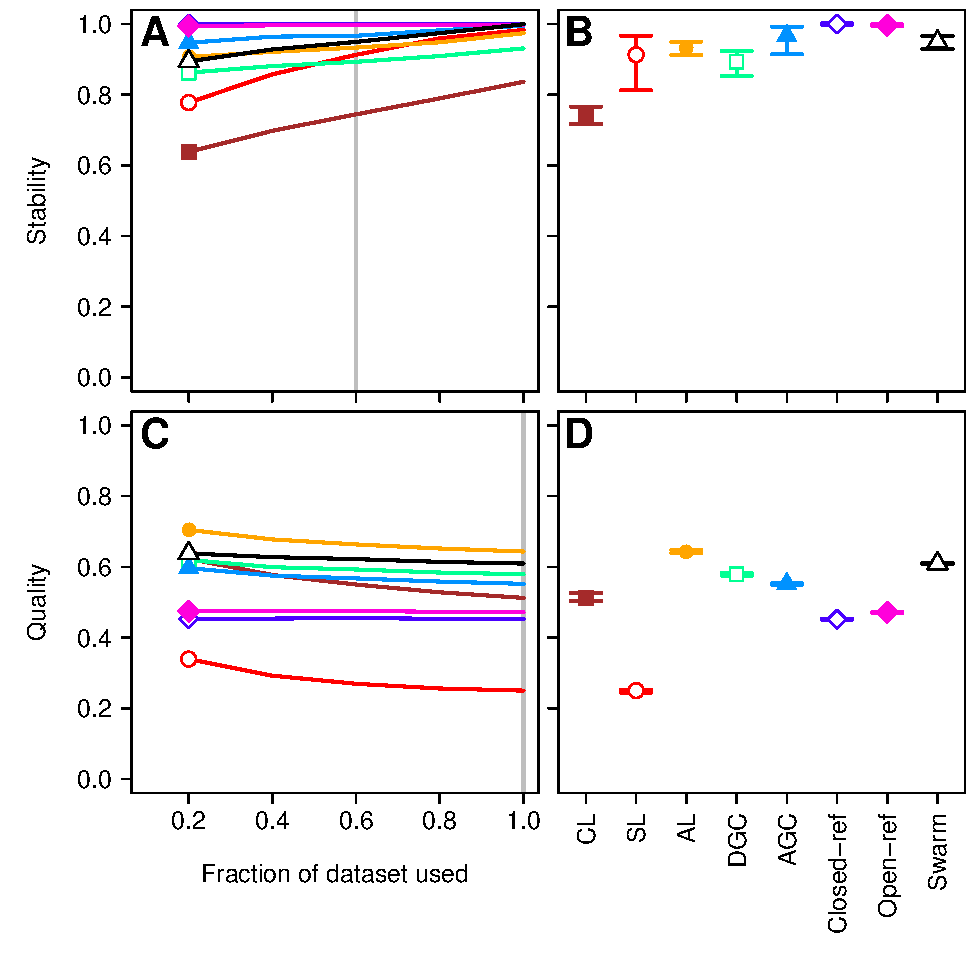
\includepdf{results/figures/figure_1.pdf}
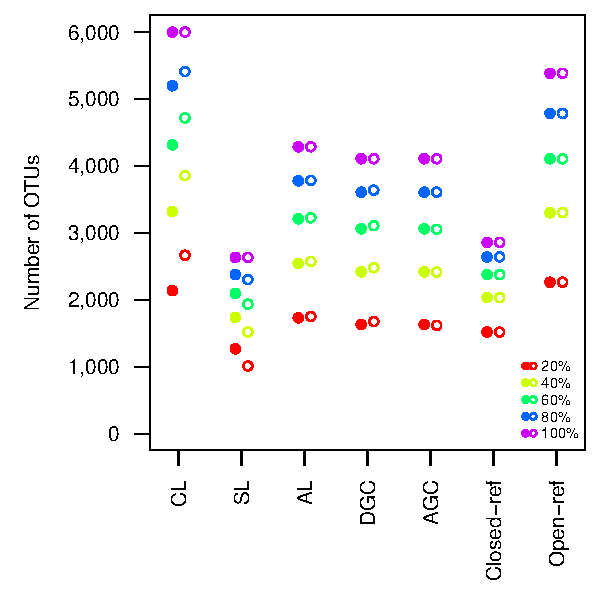
\includepdf{results/figures/figure_2.pdf}
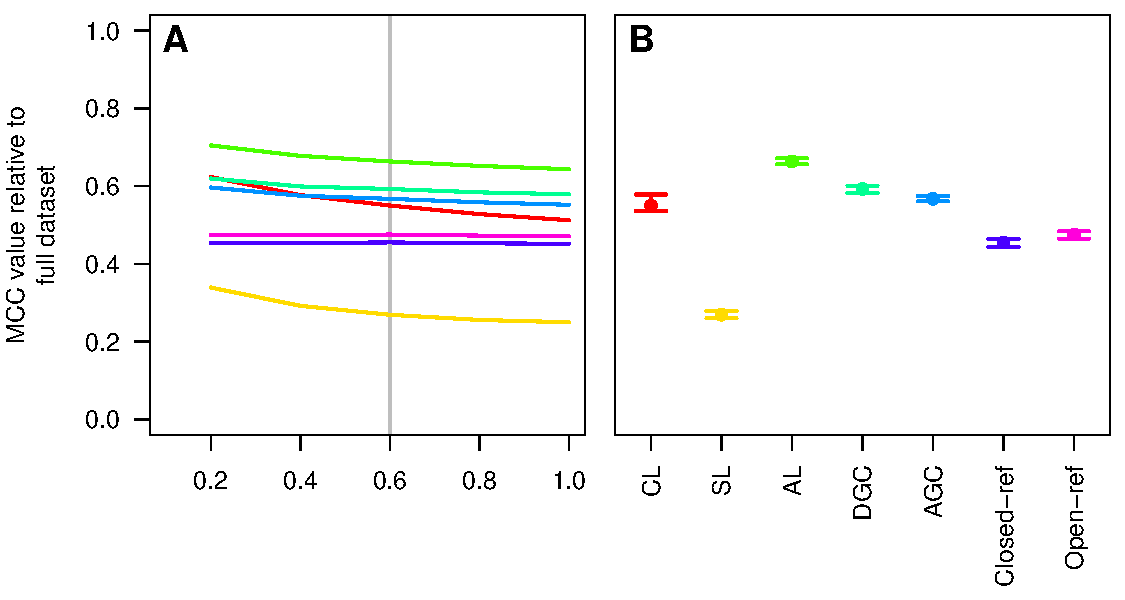
\includepdf{results/figures/figure_3.pdf}
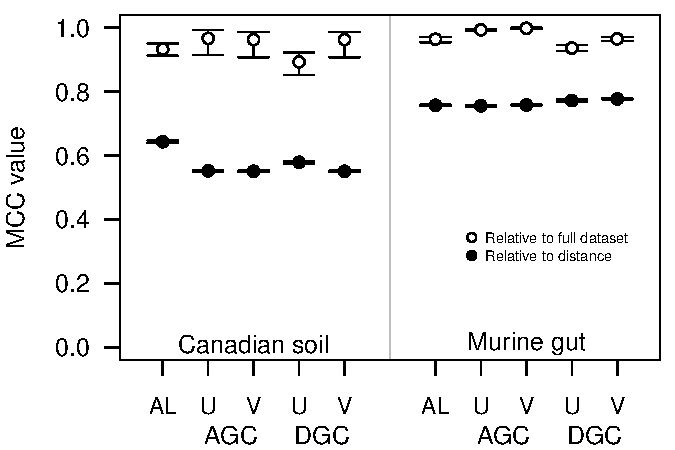
\includepdf{results/figures/figure_4.pdf}

\newpage

\hyperdef{}{references}{\label{references}}
\subsection*{References}\label{references}
\addcontentsline{toc}{subsection}{References}

\hyperdef{}{ref-Anderson2001}{\label{ref-Anderson2001}}
Anderson MJ. 2001. A new method for non-parametric multivariate analysis
of variance. \emph{Austral Ecology} 26:32--46. DOI:
\url{http://doi.org/10.1111/j.1442-9993.2001.01070.pp.x}.

\hyperdef{}{ref-Barriuso2011}{\label{ref-Barriuso2011}}
Barriuso J., Valverde JR., Mellado RP. 2011. Estimation of bacterial
diversity using next generation sequencing of 16S rDNA: A comparison of
different workflows. \emph{BMC Bioinformatics} 12:473. DOI:
\url{http://doi.org/10.1186/1471-2105-12-473}.

\hyperdef{}{ref-Bonder2012}{\label{ref-Bonder2012}}
Bonder MJ., Abeln S., Zaura E., Brandt BW. 2012. Comparing clustering
and pre-processing in taxonomy analysis. \emph{Bioinformatics}
28:2891--2897. DOI: \url{http://doi.org/10.1093/bioinformatics/bts552}.

\hyperdef{}{ref-Cai2011}{\label{ref-Cai2011}}
Cai Y., Sun Y. 2011. ESPRIT-tree: Hierarchical clustering analysis of
millions of 16S rRNA pyrosequences in quasilinear computational time.
\emph{Nucleic Acids Research} 39:e95--e95. DOI:
\url{http://doi.org/10.1093/nar/gkr349}.

\hyperdef{}{ref-Caporaso2010}{\label{ref-Caporaso2010}}
Caporaso JG., Kuczynski J., Stombaugh J., Bittinger K., Bushman FD.,
Costello EK., Fierer N., Peña AG., Goodrich JK., Gordon JI., Huttley
GA., Kelley ST., Knights D., Koenig JE., Ley RE., Lozupone CA., McDonald
D., Muegge BD., Pirrung M., Reeder J., Sevinsky JR., Turnbaugh PJ.,
Walters WA., Widmann J., Yatsunenko T., Zaneveld J., Knight R. 2010.
QIIME allows analysis of high-throughput community sequencing data.
\emph{Nature Methods} 7:335--336. DOI:
\url{http://doi.org/10.1038/nmeth.f.303}.

\hyperdef{}{ref-Chen2013}{\label{ref-Chen2013}}
Chen W., Zhang CK., Cheng Y., Zhang S., Zhao H. 2013. A comparison of
methods for clustering 16S rRNA sequences into OTUs. \emph{PLoS ONE}
8:e70837. DOI: \url{http://doi.org/10.1371/journal.pone.0070837}.

\hyperdef{}{ref-eddelbuettel2013seamless}{\label{ref-eddelbuettel2013seamless}}
Eddelbuettel D. 2013. \emph{Seamless R and C++ integration with Rcpp}.
New York: Springer.

\hyperdef{}{ref-Edgar2010}{\label{ref-Edgar2010}}
Edgar RC. 2010. Search and clustering orders of magnitude faster than
BLAST. \emph{Bioinformatics} 26:2460--2461. DOI:
\url{http://doi.org/10.1093/bioinformatics/btq461}.

\hyperdef{}{ref-Edgar2011}{\label{ref-Edgar2011}}
Edgar RC., Haas BJ., Clemente JC., Quince C., Knight R. 2011. UCHIME
improves sensitivity and speed of chimera detection.
\emph{Bioinformatics} 27:2194--2200. DOI:
\url{http://doi.org/10.1093/bioinformatics/btr381}.

\hyperdef{}{ref-Edgar2013}{\label{ref-Edgar2013}}
Edgar RC. 2013. UPARSE: Highly accurate OTU sequences from microbial
amplicon reads. \emph{Nature Methods} 10:996--998. DOI:
\url{http://doi.org/10.1038/nmeth.2604}.

\hyperdef{}{ref-Gilbert2011}{\label{ref-Gilbert2011}}
Gilbert JA., Steele JA., Caporaso JG., Steinbrück L., Reeder J.,
Temperton B., Huse S., McHardy AC., Knight R., Joint I., Somerfield P.,
Fuhrman JA., Field D. 2011. Defining seasonal marine microbial community
dynamics. \emph{The ISME Journal} 6:298--308. DOI:
\url{http://doi.org/10.1038/ismej.2011.107}.

\hyperdef{}{ref-Hamady2009}{\label{ref-Hamady2009}}
Hamady M., Lozupone C., Knight R. 2009. Fast UniFrac: Facilitating
high-throughput phylogenetic analyses of microbial communities including
analysis of pyrosequencing and PhyloChip data. \emph{The ISME Journal}
4:17--27. DOI: \url{http://doi.org/10.1038/ismej.2009.97}.

\hyperdef{}{ref-He2015}{\label{ref-He2015}}
He Y., Caporaso JG., Jiang X-T., Sheng H-F., Huse SM., Rideout JR.,
Edgar RC., Kopylova E., Walters WA., Knight R., Zhou H-W. 2015.
Stability of operational taxonomic units: An important but neglected
property for analyzing microbial diversity. \emph{Microbiome} 3. DOI:
\url{http://doi.org/10.1186/s40168-015-0081-x}.

\hyperdef{}{ref-Huse2010}{\label{ref-Huse2010}}
Huse SM., Welch DM., Morrison HG., Sogin ML. 2010. Ironing out the
wrinkles in the rare biosphere through improved OTU clustering.
\emph{Environmental Microbiology} 12:1889--1898. DOI:
\url{http://doi.org/10.1111/j.1462-2920.2010.02193.x}.

\hyperdef{}{ref-Huttenhower2012}{\label{ref-Huttenhower2012}}
Huttenhower C., Gevers D., Knight R., Abubucker S., Badger JH.,
Chinwalla AT., Creasy HH., Earl AM., FitzGerald MG., Fulton RS., Giglio
MG., Hallsworth-Pepin K., Lobos EA., Madupu R., Magrini V., Martin JC.,
Mitreva M., Muzny DM., Sodergren EJ., Versalovic J., Wollam AM., Worley
KC., Wortman JR., Young SK., Zeng Q., Aagaard KM., Abolude OO.,
Allen-Vercoe E., Alm EJ., Alvarado L., Andersen GL., Anderson S.,
Appelbaum E., Arachchi HM., Armitage G., Arze CA., Ayvaz T., Baker CC.,
Begg L., Belachew T., Bhonagiri V., Bihan M., Blaser MJ., Bloom T.,
Bonazzi V., Brooks JP., Buck GA., Buhay CJ., Busam DA., Campbell JL.,
Canon SR., Cantarel BL., Chain PSG., Chen I-MA., Chen L., Chhibba S.,
Chu K., Ciulla DM., Clemente JC., Clifton SW., Conlan S., Crabtree J.,
Cutting MA., Davidovics NJ., Davis CC., DeSantis TZ., Deal C.,
Delehaunty KD., Dewhirst FE., Deych E., Ding Y., Dooling DJ., Dugan SP.,
Dunne WM., Durkin AS., Edgar RC., Erlich RL., Farmer CN., Farrell RM.,
Faust K., Feldgarden M., Felix VM., Fisher S., Fodor AA., Forney LJ.,
Foster L., Francesco VD., Friedman J., Friedrich DC., Fronick CC.,
Fulton LL., Gao H., Garcia N., Giannoukos G., Giblin C., Giovanni MY.,
Goldberg JM., Goll J., Gonzalez A., Griggs A., Gujja S., Haake SK., Haas
BJ., Hamilton HA., Harris EL., Hepburn TA., Herter B., Hoffmann DE.,
Holder ME., Howarth C., Huang KH., Huse SM., Izard J., Jansson JK.,
Jiang H., Jordan C., Joshi V., Katancik JA., Keitel WA., Kelley ST.,
Kells C., King NB., Knights D., Kong HH., Koren O., Koren S., Kota KC.,
Kovar CL., Kyrpides NC., Rosa PSL., Lee SL., Lemon KP., Lennon N., Lewis
CM., Lewis L., Ley RE., Li K., Liolios K., Liu B., Liu Y., Lo C-C.,
Lozupone CA., Lunsford RD., Madden T., Mahurkar AA., Mannon PJ., Mardis
ER., Markowitz VM., Mavromatis K., McCorrison JM., McDonald D., McEwen
J., McGuire AL., McInnes P., Mehta T., Mihindukulasuriya KA., Miller
JR., Minx PJ., Newsham I., Nusbaum C., O'Laughlin M., Orvis J., Pagani
I., Palaniappan K., Patel SM., Pearson M., Peterson J., Podar M., Pohl
C., Pollard KS., Pop M., Priest ME., Proctor LM., Qin X., Raes J., Ravel
J., Reid JG., Rho M., Rhodes R., Riehle KP., Rivera MC.,
Rodriguez-Mueller B., Rogers Y-H., Ross MC., Russ C., Sanka RK., Sankar
P., Sathirapongsasuti JF., Schloss JA., Schloss PD., Schmidt TM., Scholz
M., Schriml L., Schubert AM., Segata N., Segre JA., Shannon WD., Sharp
RR., Sharpton TJ., Shenoy N., Sheth NU., Simone GA., Singh I., Smillie
CS., Sobel JD., Sommer DD., Spicer P., Sutton GG., Sykes SM., Tabbaa
DG., Thiagarajan M., Tomlinson CM., Torralba M., Treangen TJ., Truty
RM., Vishnivetskaya TA., Walker J., Wang L., Wang Z., Ward DV., Warren
W., Watson MA., Wellington C., Wetterstrand KA., White JR.,
Wilczek-Boney K., Wu Y., Wylie KM., Wylie T., Yandava C., Ye L., Ye Y.,
Yooseph S., Youmans BP., Zhang L., Zhou Y., Zhu Y., Zoloth L., Zucker
JD., Birren BW., Gibbs RA., Highlander SK., Methé BA., Nelson KE.,
Petrosino JF., Weinstock GM., Wilson RK., White O. 2012. Structure,
function and diversity of the healthy human microbiome. \emph{Nature}
486:207--214. DOI: \url{http://doi.org/10.1038/nature11234}.

\hyperdef{}{ref-Kim2011}{\label{ref-Kim2011}}
Kim M., Morrison M., Yu Z. 2011. Evaluation of different partial 16S
rRNA gene sequence regions for phylogenetic analysis of microbiomes.
\emph{Journal of Microbiological Methods} 84:81--87. DOI:
\url{http://doi.org/10.1016/j.mimet.2010.10.020}.

\hyperdef{}{ref-Koeppel2013}{\label{ref-Koeppel2013}}
Koeppel AF., Wu M. 2013. Surprisingly extensive mixed phylogenetic and
ecological signals among bacterial operational taxonomic units.
\emph{Nucleic Acids Research} 41:5175--5188. DOI:
\url{http://doi.org/10.1093/nar/gkt241}.

\hyperdef{}{ref-Kozich2013}{\label{ref-Kozich2013}}
Kozich JJ., Westcott SL., Baxter NT., Highlander SK., Schloss PD. 2013.
Development of a dual-index sequencing strategy and curation pipeline
for analyzing amplicon sequence data on the MiSeq Illumina sequencing
platform. \emph{Applied and Environmental Microbiology} 79:5112--5120.
DOI: \url{http://doi.org/10.1128/aem.01043-13}.

\hyperdef{}{ref-Langille2013}{\label{ref-Langille2013}}
Langille MGI., Zaneveld J., Caporaso JG., McDonald D., Knights D., Reyes
JA., Clemente JC., Burkepile DE., Thurber RLV., Knight R., Beiko RG.,
Huttenhower C. 2013. Predictive functional profiling of microbial
communities using 16S rRNA marker gene sequences. \emph{Nat Biotechnol}
31:814--821. DOI: \url{http://doi.org/10.1038/nbt.2676}.

\hyperdef{}{ref-Mah2014}{\label{ref-Mah2014}}
Mahé F., Rognes T., Quince C., Vargas C de., Dunthorn M. 2014. Swarm:
Robust and fast clustering method for amplicon-based studies.
\emph{PeerJ} 2:e593. DOI: \url{http://doi.org/10.7717/peerj.593}.

\hyperdef{}{ref-Matthews1975}{\label{ref-Matthews1975}}
Matthews B. 1975. Comparison of the predicted and observed secondary
structure of t4 phage lysozyme. \emph{Biochimica et Biophysica Acta
(BBA) - Protein Structure} 405:442--451. DOI:
\url{http://doi.org/10.1016/0005-2795(75)90109-9}.

\hyperdef{}{ref-May2014}{\label{ref-May2014}}
May A., Abeln S., Crielaard W., Heringa J., Brandt BW. 2014. Unraveling
the outcome of 16S rDNA-based taxonomy analysis through mock data and
simulations. \emph{Bioinformatics} 30:1530--1538. DOI:
\url{http://doi.org/10.1093/bioinformatics/btu085}.

\hyperdef{}{ref-NavasMolina2013}{\label{ref-NavasMolina2013}}
Navas-Molina JA., Peralta-Sánchez JM., González A., McMurdie PJ.,
Vázquez-Baeza Y., Xu Z., Ursell LK., Lauber C., Zhou H., Song SJ.,
Huntley J., Ackermann GL., Berg-Lyons D., Holmes S., Caporaso JG.,
Knight R. 2013. Advancing our understanding of the human microbiome
using QIIME. In: \emph{Methods in enzymology}. Elsevier BV, 371--444.
DOI: \url{http://doi.org/10.1016/b978-0-12-407863-5.00019-8}.

\hyperdef{}{ref-ooms2014jsonlite}{\label{ref-ooms2014jsonlite}}
Ooms J. 2014. The jsonlite package: A practical and consistent mapping
between JSON data and R objects. \emph{arXiv:1403.2805 {[}stat.CO{]}}.

\hyperdef{}{ref-Preheim2013}{\label{ref-Preheim2013}}
Preheim SP., Perrotta AR., Martin-Platero AM., Gupta A., Alm EJ. 2013.
Distribution-based clustering: Using ecology to refine the operational
taxonomic unit. \emph{Applied and Environmental Microbiology}
79:6593--6603. DOI: \url{http://doi.org/10.1128/aem.00342-13}.

\hyperdef{}{ref-Pruesse2007}{\label{ref-Pruesse2007}}
Pruesse E., Quast C., Knittel K., Fuchs BM., Ludwig W., Peplies J.,
Glockner FO. 2007. SILVA: A comprehensive online resource for quality
checked and aligned ribosomal RNA sequence data compatible with ARB.
\emph{Nucleic Acids Research} 35:7188--7196. DOI:
\url{http://doi.org/10.1093/nar/gkm864}.

\hyperdef{}{ref-language2015}{\label{ref-language2015}}
R Core Team. 2015. R: A language and environment for statistical
computing.

\hyperdef{}{ref-Rideout2014}{\label{ref-Rideout2014}}
Rideout JR., He Y., Navas-Molina JA., Walters WA., Ursell LK., Gibbons
SM., Chase J., McDonald D., Gonzalez A., Robbins-Pianka A., Clemente
JC., Gilbert JA., Huse SM., Zhou H-W., Knight R., Caporaso JG. 2014.
Subsampled open-reference clustering creates consistent, comprehensive
OTU definitions and scales to billions of sequences. \emph{PeerJ}
2:e545. DOI: \url{http://doi.org/10.7717/peerj.545}.

\hyperdef{}{ref-Roesch2007}{\label{ref-Roesch2007}}
Roesch LFW., Fulthorpe RR., Riva A., Casella G., Hadwin AKM., Kent AD.,
Daroub SH., Camargo FAO., Farmerie WG., Triplett EW. 2007.
Pyrosequencing enumerates and contrasts soil microbial diversity.
\emph{The ISME Journal}. DOI:
\url{http://doi.org/10.1038/ismej.2007.53}.

\hyperdef{}{ref-Rognes2015}{\label{ref-Rognes2015}}
Rognes T., Mahé F., Flouri T., McDonald; D. 2015. Vsearch: VSEARCH
1.4.0. DOI: \url{http://doi.org/10.5281/zenodo.31443}.

\hyperdef{}{ref-Schloss2009}{\label{ref-Schloss2009}}
Schloss PD., Westcott SL., Ryabin T., Hall JR., Hartmann M., Hollister
EB., Lesniewski RA., Oakley BB., Parks DH., Robinson CJ., Sahl JW.,
Stres B., Thallinger GG., Horn DJV., Weber CF. 2009. Introducing mothur:
Open-source, platform-independent, community-supported software for
describing and comparing microbial communities. \emph{Applied and
Environmental Microbiology} 75:7537--7541. DOI:
\url{http://doi.org/10.1128/aem.01541-09}.

\hyperdef{}{ref-Schloss2010}{\label{ref-Schloss2010}}
Schloss PD. 2010. The effects of alignment quality, distance calculation
method, sequence filtering, and region on the analysis of 16S rRNA
gene-based studies. \emph{PLoS Comput Biol} 6:e1000844. DOI:
\url{http://doi.org/10.1371/journal.pcbi.1000844}.

\hyperdef{}{ref-Schloss2012Stabilization}{\label{ref-Schloss2012Stabilization}}
Schloss PD., Schubert AM., Zackular JP., Iverson KD., Young VB.,
Petrosino JF. 2012. Stabilization of the murine gut microbiome following
weaning. \emph{Gut Microbes} 3:383--393. DOI:
\url{http://doi.org/10.4161/gmic.21008}.

\hyperdef{}{ref-Schloss2012Secondary}{\label{ref-Schloss2012Secondary}}
Schloss PD. 2012. Secondary structure improves OTU assignments of 16S
rRNA gene sequences. \emph{The ISME Journal} 7:457--460. DOI:
\url{http://doi.org/10.1038/ismej.2012.102}.

\hyperdef{}{ref-Schloss2011Assessing}{\label{ref-Schloss2011Assessing}}
Schloss PD., Westcott SL. 2011. Assessing and improving methods used in
operational taxonomic unit-based approaches for 16S rRNA gene sequence
analysis. \emph{Applied and Environmental Microbiology} 77:3219--3226.
DOI: \url{http://doi.org/10.1128/aem.02810-10}.

\hyperdef{}{ref-Schloss2011Reducing}{\label{ref-Schloss2011Reducing}}
Schloss PD., Gevers D., Westcott SL. 2011. Reducing the effects of PCR
amplification and sequencing artifacts on 16S rRNA-based studies.
\emph{PLoS ONE} 6:e27310. DOI:
\url{http://doi.org/10.1371/journal.pone.0027310}.

\hyperdef{}{ref-Schmidt2014Ecological}{\label{ref-Schmidt2014Ecological}}
Schmidt TSB., Rodrigues JFM., Mering C von. 2014a. Ecological
consistency of SSU rRNA-based operational taxonomic units at a global
scale. \emph{PLoS Comput Biol} 10:e1003594. DOI:
\url{http://doi.org/10.1371/journal.pcbi.1003594}.

\hyperdef{}{ref-Schmidt2014Limits}{\label{ref-Schmidt2014Limits}}
Schmidt TSB., Rodrigues JFM., Mering C von. 2014b. Limits to robustness
and reproducibility in the demarcation of operational taxonomic units.
\emph{Environ Microbiol} 17:1689--1706. DOI:
\url{http://doi.org/10.1111/1462-2920.12610}.

\hyperdef{}{ref-Schubert2015}{\label{ref-Schubert2015}}
Schubert AM., Sinani H., Schloss PD. 2015. Antibiotic-induced
alterations of the murine gut microbiota and subsequent effects on
colonization resistance against *clostridium difficile*. \emph{mBio}
6:e00974--15. DOI: \url{http://doi.org/10.1128/mbio.00974-15}.

\hyperdef{}{ref-Shade2013}{\label{ref-Shade2013}}
Shade A., Klimowicz AK., Spear RN., Linske M., Donato JJ., Hogan CS.,
McManus PS., Handelsman J. 2013. Streptomycin application has no
detectable effect on bacterial community structure in apple orchard
soil. \emph{Applied and Environmental Microbiology} 79:6617--6625. DOI:
\url{http://doi.org/10.1128/aem.02017-13}.

\hyperdef{}{ref-Sun2009}{\label{ref-Sun2009}}
Sun Y., Cai Y., Liu L., Yu F., Farrell ML., McKendree W., Farmerie W.
2009. ESPRIT: Estimating species richness using large collections of 16S
rRNA pyrosequences. \emph{Nucleic Acids Research} 37:e76--e76. DOI:
\url{http://doi.org/10.1093/nar/gkp285}.

\hyperdef{}{ref-Sun2011}{\label{ref-Sun2011}}
Sun Y., Cai Y., Huse SM., Knight R., Farmerie WG., Wang X., Mai V. 2011.
A large-scale benchmark study of existing algorithms for
taxonomy-independent microbial community analysis. \emph{Briefings in
Bioinformatics} 13:107--121. DOI:
\url{http://doi.org/10.1093/bib/bbr009}.

\hyperdef{}{ref-Wang2007}{\label{ref-Wang2007}}
Wang Q., Garrity GM., Tiedje JM., Cole JR. 2007. Naive bayesian
classifier for rapid assignment of rRNA sequences into the new bacterial
taxonomy. \emph{Applied and Environmental Microbiology} 73:5261--5267.
DOI: \url{http://doi.org/10.1128/aem.00062-07}.

\hyperdef{}{ref-White2010}{\label{ref-White2010}}
White JR., Navlakha S., Nagarajan N., Ghodsi M-R., Kingsford C., Pop M.
2010. Alignment and clustering of phylogenetic markers - implications
for microbial diversity studies. \emph{BMC Bioinformatics} 11:152. DOI:
\url{http://doi.org/10.1186/1471-2105-11-152}.

\hyperdef{}{ref-winter2015rentrez}{\label{ref-winter2015rentrez}}
Winter D., Chamberlain S., Guangchun H. 2015. Rentrez 1.0.0. DOI:
\url{http://doi.org/10.5281/zenodo.32420}.

\hyperdef{}{ref-xie2013dynamic}{\label{ref-xie2013dynamic}}
Xie Y. 2013. \emph{Dynamic documents with R and knitr}. Boca Raton,
Florida: Chapman; Hall/CRC.

\hyperdef{}{ref-Zackular2015}{\label{ref-Zackular2015}}
Zackular JP., Baxter NT., Chen GY., Schloss PD. 2015. Manipulation of
the gut microbiota reveals role in colon tumorigenesis. \emph{mSphere}
1:e00001--15. DOI: \url{http://doi.org/10.1128/mSphere.00001-15}.

\end{document}
